\documentclass{standalone}
\usepackage{tikz}
\begin{document}

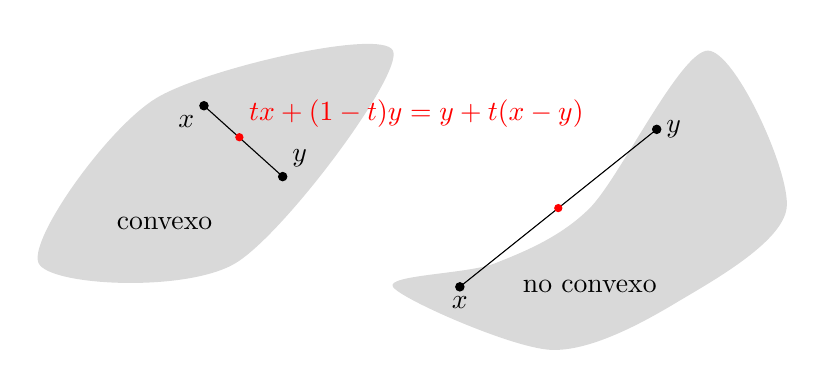
\begin{tikzpicture}[>=latex]
	\fill [gray, opacity=0.3] plot [smooth cycle] coordinates{(-0.5,1.3) (1,3.4) (4,4) (2,1.3)};
	\node at (1.1,1.8) {convexo};
	\filldraw [shift={(-0.5,-0.5)}] (2.1,3.8) circle (1.5pt) node [below left] {\(x\)} -- (3.1,2.9) circle (1.5pt) node [above right] {\(y\)};
	\fill [red] (2.05,2.9) circle (1.5pt) node [above right] {\(tx+(1-t) y = y + t(x-y)\)};
	\begin{scope}[xshift=-1cm]
		\fill [gray, opacity=0.3, xshift=2cm] plot [smooth cycle] coordinates{(3,1) (4.3,1.3) (5.5,2) (7,4) (8,2) (6.6,0.8) (5,0.2)};
		\node at (7.5,1) {no convexo};
		\filldraw [xshift=-6.5mm] (6.5,1) circle (1.5pt) node [below] {\(x\)} -- (9,3) circle (1.5pt) node [right] {\(y\)};
		\fill [red] (7.1,2) circle (1.5pt);
	\end{scope}
\end{tikzpicture}

\end{document}
